\documentclass[twoside]{book}

% Packages required by doxygen
\usepackage{calc}
\usepackage{doxygen}
\usepackage{graphicx}
\usepackage[utf8]{inputenc}
\usepackage{makeidx}
\usepackage{multicol}
\usepackage{multirow}
\usepackage{textcomp}
\usepackage[table]{xcolor}

% Font selection
\usepackage[T1]{fontenc}
\usepackage{mathptmx}
\usepackage[scaled=.90]{helvet}
\usepackage{courier}
\usepackage{amssymb}
\usepackage{sectsty}
\renewcommand{\familydefault}{\sfdefault}
\allsectionsfont{%
  \fontseries{bc}\selectfont%
  \color{darkgray}%
}
\renewcommand{\DoxyLabelFont}{%
  \fontseries{bc}\selectfont%
  \color{darkgray}%
}

% Page & text layout
\usepackage{geometry}
\geometry{%
  a4paper,%
  top=2.5cm,%
  bottom=2.5cm,%
  left=2.5cm,%
  right=2.5cm%
}
\tolerance=750
\hfuzz=15pt
\hbadness=750
\setlength{\emergencystretch}{15pt}
\setlength{\parindent}{0cm}
\setlength{\parskip}{0.2cm}
\makeatletter
\renewcommand{\paragraph}{%
  \@startsection{paragraph}{4}{0ex}{-1.0ex}{1.0ex}{%
    \normalfont\normalsize\bfseries\SS@parafont%
  }%
}
\renewcommand{\subparagraph}{%
  \@startsection{subparagraph}{5}{0ex}{-1.0ex}{1.0ex}{%
    \normalfont\normalsize\bfseries\SS@subparafont%
  }%
}
\makeatother

% Headers & footers
\usepackage{fancyhdr}
\pagestyle{fancyplain}
\fancyhead[LE]{\fancyplain{}{\bfseries\thepage}}
\fancyhead[CE]{\fancyplain{}{}}
\fancyhead[RE]{\fancyplain{}{\bfseries\leftmark}}
\fancyhead[LO]{\fancyplain{}{\bfseries\rightmark}}
\fancyhead[CO]{\fancyplain{}{}}
\fancyhead[RO]{\fancyplain{}{\bfseries\thepage}}
\fancyfoot[LE]{\fancyplain{}{}}
\fancyfoot[CE]{\fancyplain{}{}}
\fancyfoot[RE]{\fancyplain{}{\bfseries\scriptsize Generated on Wed Jun 19 2013 11:39:05 for Dungeon Brothers by Doxygen }}
\fancyfoot[LO]{\fancyplain{}{\bfseries\scriptsize Generated on Wed Jun 19 2013 11:39:05 for Dungeon Brothers by Doxygen }}
\fancyfoot[CO]{\fancyplain{}{}}
\fancyfoot[RO]{\fancyplain{}{}}
\renewcommand{\footrulewidth}{0.4pt}
\renewcommand{\chaptermark}[1]{%
  \markboth{#1}{}%
}
\renewcommand{\sectionmark}[1]{%
  \markright{\thesection\ #1}%
}

% Indices & bibliography
\usepackage{natbib}
\usepackage[titles]{tocloft}
\setcounter{tocdepth}{3}
\setcounter{secnumdepth}{5}
\makeindex

% Hyperlinks (required, but should be loaded last)
\usepackage{ifpdf}
\ifpdf
  \usepackage[pdftex,pagebackref=true]{hyperref}
\else
  \usepackage[ps2pdf,pagebackref=true]{hyperref}
\fi
\hypersetup{%
  colorlinks=true,%
  linkcolor=blue,%
  citecolor=blue,%
  unicode%
}

% Custom commands
\newcommand{\clearemptydoublepage}{%
  \newpage{\pagestyle{empty}\cleardoublepage}%
}


%===== C O N T E N T S =====

\begin{document}

% Titlepage & ToC
\hypersetup{pageanchor=false}
\pagenumbering{roman}
\begin{titlepage}
\vspace*{7cm}
\begin{center}%
{\Large Dungeon Brothers }\\
\vspace*{1cm}
{\large Generated by Doxygen 1.8.4}\\
\vspace*{0.5cm}
{\small Wed Jun 19 2013 11:39:05}\\
\end{center}
\end{titlepage}
\clearemptydoublepage
\tableofcontents
\clearemptydoublepage
\pagenumbering{arabic}
\hypersetup{pageanchor=true}

%--- Begin generated contents ---
\chapter{Dungeon\-Brothers}
\label{md_C:_Users_BW.KEE_Documents_GitHub_DungeonBrothers_README}
\hypertarget{md_C:_Users_BW.KEE_Documents_GitHub_DungeonBrothers_README}{}
A cool opensource game inspired on a classic amiga platform game called Yo Joe by Hudsonsoft. This engine is written in native C++ using the S\-D\-L Library. Developed on Win32 in Codeblocks/\-Ming\-W but should be easy to port to other platforms.

Goals (momentary)\-: \begin{DoxyVerb}- Fast and exciting gameplay
- Tile based engine
- Paralax scrolling background
- Built in level editor
- Keyboard and Joystick input
- 2 Player Mode
- Original amiga / tracker style music and audio FX
- Aprox. 10 levels in different theme's
\end{DoxyVerb}


Team members\-: \begin{DoxyVerb}Name            Real name           Function
=====================================================================================
Defcon8         Bastiaan de Waard   Programmer / Music / Audio FX
\end{DoxyVerb}


We are looking forward to meet new team members\-: \begin{DoxyVerb}- Programmers
- Graphic designers
- Level designers
\end{DoxyVerb}


Contact\-: \href{mailto:info@bastiaandewaard.com}{\tt info@bastiaandewaard.\-com} 
\chapter{Hierarchical Index}
\section{Class Hierarchy}
This inheritance list is sorted roughly, but not completely, alphabetically\-:\begin{DoxyCompactList}
\item \contentsline{section}{c\-Camera}{\pageref{classc_camera}}{}
\item \contentsline{section}{c\-Debug}{\pageref{classc_debug}}{}
\item \contentsline{section}{c\-Game}{\pageref{classc_game}}{}
\item \contentsline{section}{c\-Pencil}{\pageref{classc_pencil}}{}
\item \contentsline{section}{c\-Screen\-Row}{\pageref{classc_screen_row}}{}
\item \contentsline{section}{c\-Sprite}{\pageref{classc_sprite}}{}
\item \contentsline{section}{c\-Sprite\-Layer}{\pageref{classc_sprite_layer}}{}
\item \contentsline{section}{i\-Level\-Object}{\pageref{classi_level_object}}{}
\begin{DoxyCompactList}
\item \contentsline{section}{c\-Enemy}{\pageref{classc_enemy}}{}
\item \contentsline{section}{c\-Level\-Object}{\pageref{classc_level_object}}{}
\begin{DoxyCompactList}
\item \contentsline{section}{c\-Player}{\pageref{classc_player}}{}
\end{DoxyCompactList}
\end{DoxyCompactList}
\end{DoxyCompactList}

\chapter{Class Index}
\section{Class List}
Here are the classes, structs, unions and interfaces with brief descriptions\-:\begin{DoxyCompactList}
\item\contentsline{section}{\hyperlink{classc_debug}{c\-Debug} }{\pageref{classc_debug}}{}
\item\contentsline{section}{\hyperlink{classc_game}{c\-Game} }{\pageref{classc_game}}{}
\item\contentsline{section}{\hyperlink{classc_pencil}{c\-Pencil} }{\pageref{classc_pencil}}{}
\item\contentsline{section}{\hyperlink{classc_screen_row}{c\-Screen\-Row} }{\pageref{classc_screen_row}}{}
\item\contentsline{section}{\hyperlink{classc_sprite}{c\-Sprite} }{\pageref{classc_sprite}}{}
\item\contentsline{section}{\hyperlink{classc_sprite_layer}{c\-Sprite\-Layer} }{\pageref{classc_sprite_layer}}{}
\end{DoxyCompactList}

\chapter{Class Documentation}
\hypertarget{classc_camera}{\section{c\-Camera Class Reference}
\label{classc_camera}\index{c\-Camera@{c\-Camera}}
}
\subsection*{Public Attributes}
\begin{DoxyCompactItemize}
\item 
\hypertarget{classc_camera_a62e36b937336e6bd339b651a770c7ee1}{int {\bfseries up}}\label{classc_camera_a62e36b937336e6bd339b651a770c7ee1}

\item 
\hypertarget{classc_camera_af721aac68a5f438be50a9ae057433356}{int {\bfseries right}}\label{classc_camera_af721aac68a5f438be50a9ae057433356}

\item 
\hypertarget{classc_camera_a34d7c56be2d8e4dbbd1ab72a74575945}{int {\bfseries down}}\label{classc_camera_a34d7c56be2d8e4dbbd1ab72a74575945}

\item 
\hypertarget{classc_camera_a3570540278b4673d39743fcac2bac670}{int {\bfseries left}}\label{classc_camera_a3570540278b4673d39743fcac2bac670}

\item 
\hypertarget{classc_camera_a15ecc854c43d9a8a48e0c42e75a14678}{int {\bfseries none}}\label{classc_camera_a15ecc854c43d9a8a48e0c42e75a14678}

\item 
\hypertarget{classc_camera_a80d81977a55a45291c663420a61c9993}{int {\bfseries X}}\label{classc_camera_a80d81977a55a45291c663420a61c9993}

\item 
\hypertarget{classc_camera_a158414cc2aa9a0e08087e91e876709f9}{int {\bfseries Y}}\label{classc_camera_a158414cc2aa9a0e08087e91e876709f9}

\item 
\hypertarget{classc_camera_a61ac25e1d39c85331aa8dac91b5dda63}{int {\bfseries Direction}}\label{classc_camera_a61ac25e1d39c85331aa8dac91b5dda63}

\end{DoxyCompactItemize}


The documentation for this class was generated from the following files\-:\begin{DoxyCompactItemize}
\item 
C\-:/\-Users/\-B\-W.\-K\-E\-E/\-Documents/\-Git\-Hub/\-Dungeon\-Brothers/camera.\-h\item 
C\-:/\-Users/\-B\-W.\-K\-E\-E/\-Documents/\-Git\-Hub/\-Dungeon\-Brothers/camera.\-c\end{DoxyCompactItemize}

\hypertarget{classc_debug}{\section{c\-Debug Class Reference}
\label{classc_debug}\index{c\-Debug@{c\-Debug}}
}


The documentation for this class was generated from the following files\-:\begin{DoxyCompactItemize}
\item 
C\-:/\-Users/\-B\-W.\-K\-E\-E/\-Documents/\-Git\-Hub/\-Dungeon\-Brothers/debug.\-h\item 
C\-:/\-Users/\-B\-W.\-K\-E\-E/\-Documents/\-Git\-Hub/\-Dungeon\-Brothers/debug.\-c\end{DoxyCompactItemize}

\hypertarget{classc_enemy}{\section{c\-Enemy Class Reference}
\label{classc_enemy}\index{c\-Enemy@{c\-Enemy}}
}
Inheritance diagram for c\-Enemy\-:\begin{figure}[H]
\begin{center}
\leavevmode
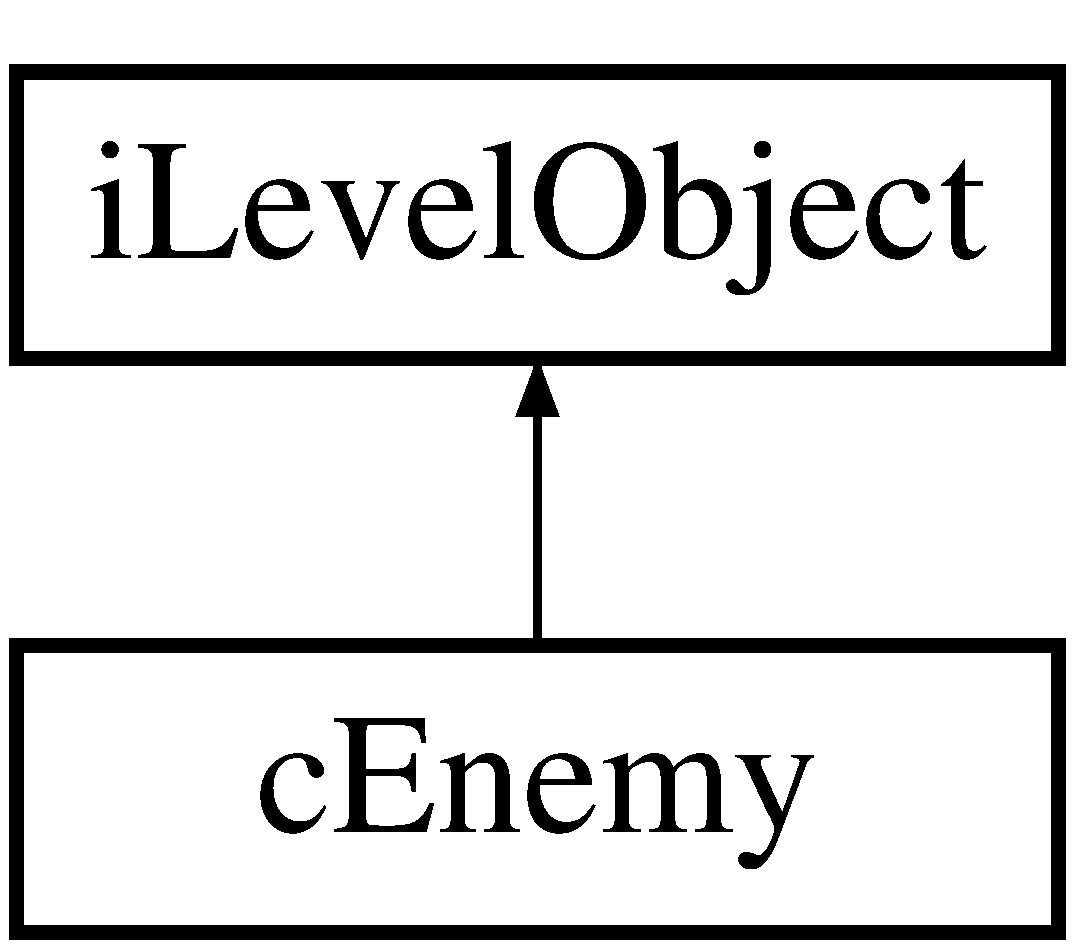
\includegraphics[height=2.000000cm]{classc_enemy}
\end{center}
\end{figure}
\subsection*{Public Member Functions}
\begin{DoxyCompactItemize}
\item 
\hypertarget{classc_enemy_a144216f8359bacaf5dd6b243d14fc0ae}{virtual void {\bfseries f\-Update} ()}\label{classc_enemy_a144216f8359bacaf5dd6b243d14fc0ae}

\end{DoxyCompactItemize}


The documentation for this class was generated from the following files\-:\begin{DoxyCompactItemize}
\item 
C\-:/\-Users/\-B\-W.\-K\-E\-E/\-Documents/\-Git\-Hub/\-Dungeon\-Brothers/enemy.\-h\item 
C\-:/\-Users/\-B\-W.\-K\-E\-E/\-Documents/\-Git\-Hub/\-Dungeon\-Brothers/enemy.\-c\end{DoxyCompactItemize}

\hypertarget{classc_game}{\section{c\-Game Class Reference}
\label{classc_game}\index{c\-Game@{c\-Game}}
}
\subsection*{Public Types}
\begin{DoxyCompactItemize}
\item 
enum {\bfseries e\-Data\-Type} \{ {\bfseries S\-P\-R\-I\-T\-E\-L\-A\-Y\-E\-R}, 
{\bfseries S\-P\-R\-I\-T\-E}
 \}
\end{DoxyCompactItemize}
\subsection*{Public Member Functions}
\begin{DoxyCompactItemize}
\item 
\hypertarget{classc_game_aacd692d88029466a0ae346b022f5c7b4}{void {\bfseries Start} ()}\label{classc_game_aacd692d88029466a0ae346b022f5c7b4}

\item 
\hypertarget{classc_game_a3f1b9d09b77e67cdcb1c22492f3400a0}{{\bfseries c\-Game} (int i\-Scr\-Width, int i\-Scr\-Height)}\label{classc_game_a3f1b9d09b77e67cdcb1c22492f3400a0}

\end{DoxyCompactItemize}
\subsection*{Public Attributes}
\begin{DoxyCompactItemize}
\item 
\hypertarget{classc_game_a93aa23090d4531fffe232507f762b7e8}{e\-Data\-Type {\bfseries Type}}\label{classc_game_a93aa23090d4531fffe232507f762b7e8}

\end{DoxyCompactItemize}


The documentation for this class was generated from the following files\-:\begin{DoxyCompactItemize}
\item 
C\-:/\-Users/\-B\-W.\-K\-E\-E/\-Documents/\-Git\-Hub/\-Dungeon\-Brothers/game.\-h\item 
C\-:/\-Users/\-B\-W.\-K\-E\-E/\-Documents/\-Git\-Hub/\-Dungeon\-Brothers/gamedata.\-h\item 
C\-:/\-Users/\-B\-W.\-K\-E\-E/\-Documents/\-Git\-Hub/\-Dungeon\-Brothers/game.\-c\end{DoxyCompactItemize}

\hypertarget{classc_level_object}{\section{c\-Level\-Object Class Reference}
\label{classc_level_object}\index{c\-Level\-Object@{c\-Level\-Object}}
}
Inheritance diagram for c\-Level\-Object\-:\begin{figure}[H]
\begin{center}
\leavevmode
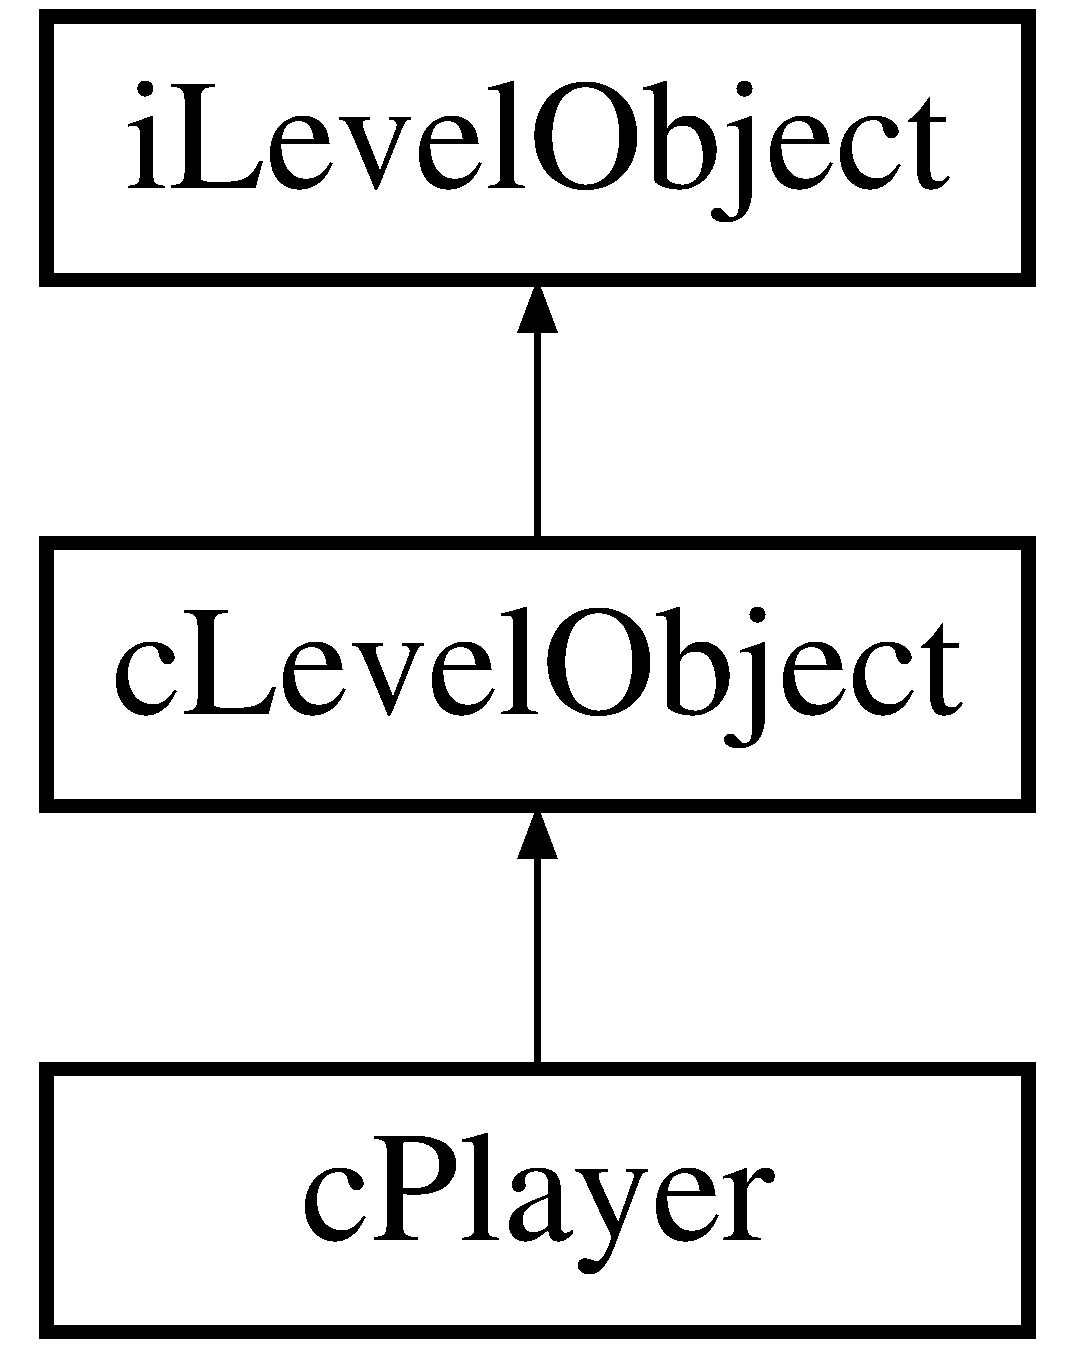
\includegraphics[height=3.000000cm]{classc_level_object}
\end{center}
\end{figure}
\subsection*{Public Member Functions}
\begin{DoxyCompactItemize}
\item 
\hypertarget{classc_level_object_a3caa9a85867d35c700ce8146e2ff2975}{{\bfseries c\-Level\-Object} (S\-D\-L\-\_\-\-Surface $\ast$screen, \hyperlink{classc_sprite_layer}{c\-Sprite\-Layer} $\ast$o\-Level\-Layer\-Ref, \hyperlink{classc_camera}{c\-Camera} $\ast$o\-Cam\-Ref, char $\ast$ch\-Tile\-Source, int i\-Sprite\-Height, int i\-Sprite\-Width, int i\-Screen\-Width\-Ref, int i\-Screen\-Height\-Ref)}\label{classc_level_object_a3caa9a85867d35c700ce8146e2ff2975}

\item 
\hypertarget{classc_level_object_ade464b941da84f307ca13e7b7ff20ff9}{virtual void {\bfseries f\-Update} ()}\label{classc_level_object_ade464b941da84f307ca13e7b7ff20ff9}

\item 
\hypertarget{classc_level_object_ab1c03ffbaef6a3b662c737758160f0d7}{void {\bfseries f\-Move\-Direction} (int i\-Direction, bool bl\-Enabled)}\label{classc_level_object_ab1c03ffbaef6a3b662c737758160f0d7}

\end{DoxyCompactItemize}
\subsection*{Public Attributes}
\begin{DoxyCompactItemize}
\item 
\hypertarget{classc_level_object_adef4d9f84d178e332e769a324eed527e}{\hyperlink{classc_sprite_layer}{c\-Sprite\-Layer} $\ast$ {\bfseries o\-Player\-Layer}}\label{classc_level_object_adef4d9f84d178e332e769a324eed527e}

\item 
\hypertarget{classc_level_object_a679fa5636166989650b6b08198812f12}{\hyperlink{classc_sprite_layer}{c\-Sprite\-Layer} $\ast$ {\bfseries o\-Level\-Layer}}\label{classc_level_object_a679fa5636166989650b6b08198812f12}

\item 
\hypertarget{classc_level_object_adb5d526afbfcf50d3884e0d6c7f97e68}{\hyperlink{classc_camera}{c\-Camera} $\ast$ {\bfseries o\-Cam}}\label{classc_level_object_adb5d526afbfcf50d3884e0d6c7f97e68}

\end{DoxyCompactItemize}


The documentation for this class was generated from the following files\-:\begin{DoxyCompactItemize}
\item 
C\-:/\-Users/\-B\-W.\-K\-E\-E/\-Documents/\-Git\-Hub/\-Dungeon\-Brothers/levelobject.\-h\item 
C\-:/\-Users/\-B\-W.\-K\-E\-E/\-Documents/\-Git\-Hub/\-Dungeon\-Brothers/levelobject.\-c\end{DoxyCompactItemize}

\hypertarget{classc_pencil}{\section{c\-Pencil Class Reference}
\label{classc_pencil}\index{c\-Pencil@{c\-Pencil}}
}
\subsection*{Public Attributes}
\begin{DoxyCompactItemize}
\item 
\hypertarget{classc_pencil_ae4e4dc8ff114ca11ff1763b56755ff2b}{int {\bfseries i\-Source\-Tile\-Row}}\label{classc_pencil_ae4e4dc8ff114ca11ff1763b56755ff2b}

\item 
\hypertarget{classc_pencil_acb8fb1c96a11eaeb2f48f4d79d1dba13}{int {\bfseries i\-Source\-Tile\-Col}}\label{classc_pencil_acb8fb1c96a11eaeb2f48f4d79d1dba13}

\end{DoxyCompactItemize}


The documentation for this class was generated from the following files\-:\begin{DoxyCompactItemize}
\item 
C\-:/\-Users/\-B\-W.\-K\-E\-E/\-Documents/\-Git\-Hub/\-Dungeon\-Brothers/pencil.\-h\item 
C\-:/\-Users/\-B\-W.\-K\-E\-E/\-Documents/\-Git\-Hub/\-Dungeon\-Brothers/pencil.\-c\end{DoxyCompactItemize}

\hypertarget{classc_player}{\section{c\-Player Class Reference}
\label{classc_player}\index{c\-Player@{c\-Player}}
}
Inheritance diagram for c\-Player\-:\begin{figure}[H]
\begin{center}
\leavevmode
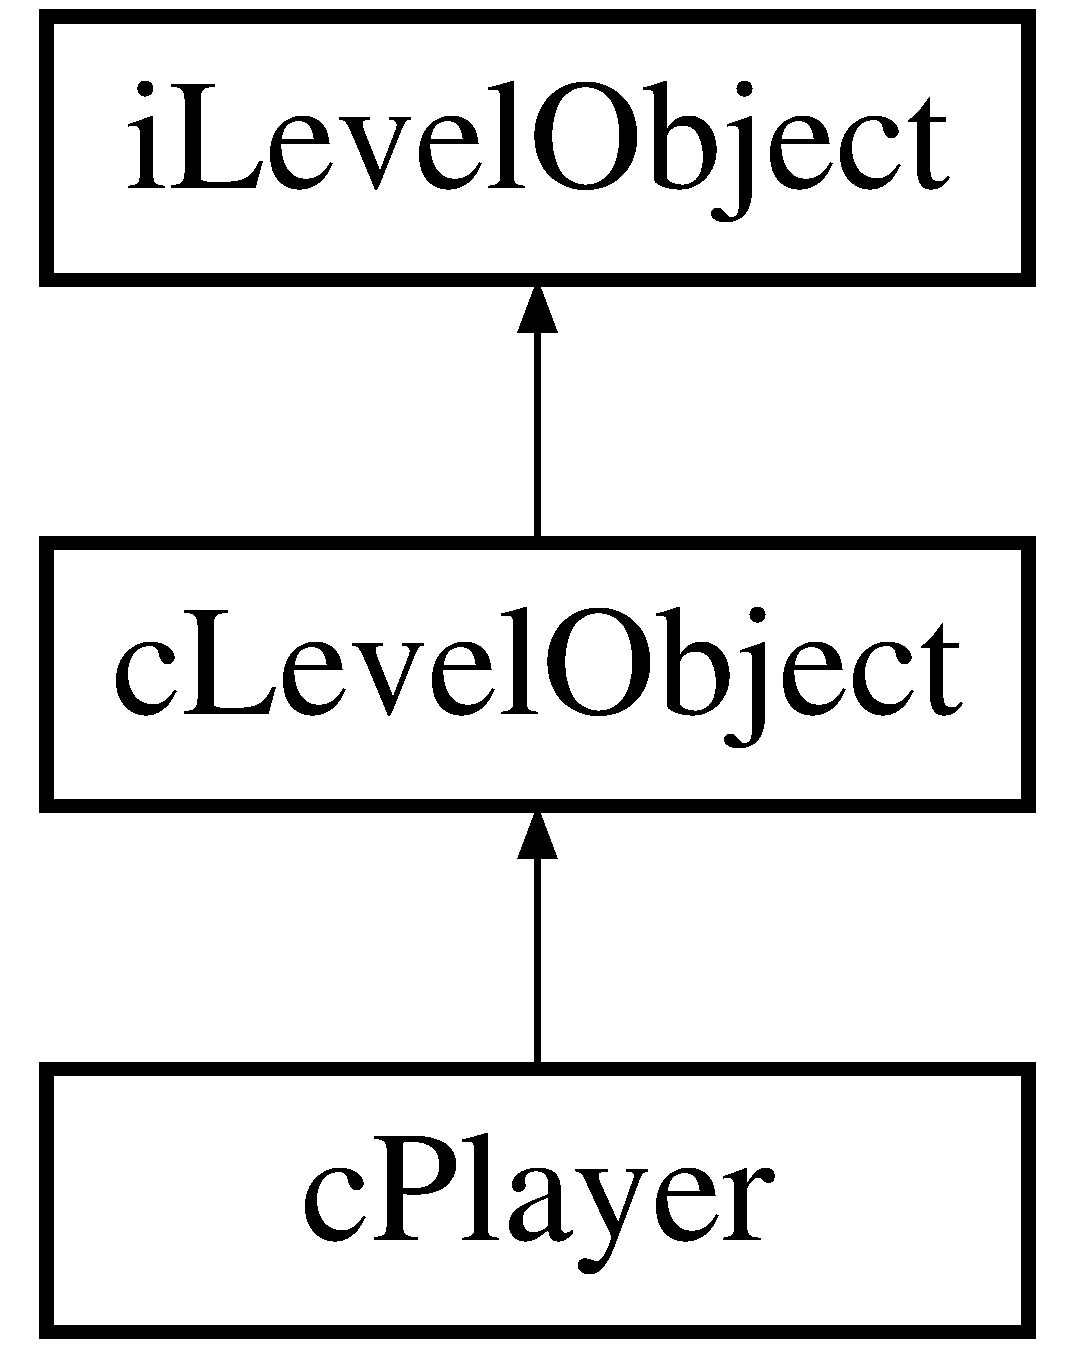
\includegraphics[height=3.000000cm]{classc_player}
\end{center}
\end{figure}
\subsection*{Additional Inherited Members}


The documentation for this class was generated from the following files\-:\begin{DoxyCompactItemize}
\item 
C\-:/\-Users/\-B\-W.\-K\-E\-E/\-Documents/\-Git\-Hub/\-Dungeon\-Brothers/player.\-h\item 
C\-:/\-Users/\-B\-W.\-K\-E\-E/\-Documents/\-Git\-Hub/\-Dungeon\-Brothers/player.\-c\end{DoxyCompactItemize}

\hypertarget{classc_screen_row}{\section{c\-Screen\-Row Class Reference}
\label{classc_screen_row}\index{c\-Screen\-Row@{c\-Screen\-Row}}
}


The documentation for this class was generated from the following files\-:\begin{DoxyCompactItemize}
\item 
C\-:/\-Users/\-B\-W.\-K\-E\-E/\-Documents/\-Git\-Hub/\-Dungeon\-Brothers/screenrow.\-h\item 
C\-:/\-Users/\-B\-W.\-K\-E\-E/\-Documents/\-Git\-Hub/\-Dungeon\-Brothers/screenrow.\-c\end{DoxyCompactItemize}

\hypertarget{classc_sprite}{\section{c\-Sprite Class Reference}
\label{classc_sprite}\index{c\-Sprite@{c\-Sprite}}
}
\subsection*{Public Member Functions}
\begin{DoxyCompactItemize}
\item 
\hypertarget{classc_sprite_a83f6cccb37f09df84aca31c6d6370fea}{void {\bfseries f\-Load} (const char $\ast$file)}\label{classc_sprite_a83f6cccb37f09df84aca31c6d6370fea}

\item 
\hypertarget{classc_sprite_a34b4cbf7e9c2bc5017628f83f9182529}{void {\bfseries f\-Render} (int i\-Col, int i\-Row, int i\-Dest\-X, int i\-Dest\-Y)}\label{classc_sprite_a34b4cbf7e9c2bc5017628f83f9182529}

\item 
\hypertarget{classc_sprite_aaae9b0ff3031c0a5d8a4e21b3d7431bc}{void {\bfseries f\-Set\-Sprite\-Width} (int i\-Pixels)}\label{classc_sprite_aaae9b0ff3031c0a5d8a4e21b3d7431bc}

\item 
\hypertarget{classc_sprite_a77fc288cc44fa79fbab13bea705146fd}{void {\bfseries f\-Set\-Sprite\-Height} (int i\-Pixels)}\label{classc_sprite_a77fc288cc44fa79fbab13bea705146fd}

\item 
\hypertarget{classc_sprite_a921d6b5c47fba92255f37aff598d102a}{void {\bfseries f\-Set\-Sprite\-Width\-Offset} (int i\-Pixels)}\label{classc_sprite_a921d6b5c47fba92255f37aff598d102a}

\item 
\hypertarget{classc_sprite_a8f50fa8cc54b0b4f0b1207c335596b3c}{void {\bfseries f\-Set\-Sprite\-Height\-Offset} (int i\-Pixels)}\label{classc_sprite_a8f50fa8cc54b0b4f0b1207c335596b3c}

\item 
\hypertarget{classc_sprite_abc08170b8a732dd2efe966f096025b3f}{void {\bfseries f\-Set\-Sprite\-Spacer} (int i\-Pixels)}\label{classc_sprite_abc08170b8a732dd2efe966f096025b3f}

\item 
\hypertarget{classc_sprite_aa98bb76898e040e1c6dae95758e073b1}{int {\bfseries f\-Get\-Sprite\-Width} ()}\label{classc_sprite_aa98bb76898e040e1c6dae95758e073b1}

\item 
\hypertarget{classc_sprite_a03228f1a93a795392d83f433e243ff07}{int {\bfseries f\-Get\-Sprite\-Height} ()}\label{classc_sprite_a03228f1a93a795392d83f433e243ff07}

\item 
\hypertarget{classc_sprite_abb0ae63b1039d3caccdff9eafe6dd282}{int {\bfseries f\-Get\-Sprite\-Width\-Offset} ()}\label{classc_sprite_abb0ae63b1039d3caccdff9eafe6dd282}

\item 
\hypertarget{classc_sprite_ab710b29658c751f2988368d438b6f27f}{int {\bfseries f\-Get\-Sprite\-Height\-Offset} ()}\label{classc_sprite_ab710b29658c751f2988368d438b6f27f}

\item 
\hypertarget{classc_sprite_a406a292a0b156ddc716c3f6a4ac62f12}{int {\bfseries f\-Get\-Sprite\-Spacer} ()}\label{classc_sprite_a406a292a0b156ddc716c3f6a4ac62f12}

\item 
\hypertarget{classc_sprite_a81cab547630d110e9015cf2f85918e51}{char $\ast$ {\bfseries f\-Get\-Tile\-Source} ()}\label{classc_sprite_a81cab547630d110e9015cf2f85918e51}

\item 
\hypertarget{classc_sprite_a200e49fcedb589fa54139dc9cbd2f07e}{void {\bfseries f\-Set\-Color\-Key} (int i\-R, int i\-G, int i\-B)}\label{classc_sprite_a200e49fcedb589fa54139dc9cbd2f07e}

\item 
\hypertarget{classc_sprite_a88cb2a43a5653ef449ee5f3974307dfc}{void {\bfseries f\-Scroll} ()}\label{classc_sprite_a88cb2a43a5653ef449ee5f3974307dfc}

\item 
\hypertarget{classc_sprite_abeebe92ab7bef34feec37b26f3ecd0a2}{{\bfseries c\-Sprite} (S\-D\-L\-\_\-\-Surface $\ast$screen)}\label{classc_sprite_abeebe92ab7bef34feec37b26f3ecd0a2}

\end{DoxyCompactItemize}


The documentation for this class was generated from the following files\-:\begin{DoxyCompactItemize}
\item 
C\-:/\-Users/\-B\-W.\-K\-E\-E/\-Documents/\-Git\-Hub/\-Dungeon\-Brothers/sprite.\-h\item 
C\-:/\-Users/\-B\-W.\-K\-E\-E/\-Documents/\-Git\-Hub/\-Dungeon\-Brothers/sprite.\-c\end{DoxyCompactItemize}

\hypertarget{classc_sprite_layer}{\section{c\-Sprite\-Layer Class Reference}
\label{classc_sprite_layer}\index{c\-Sprite\-Layer@{c\-Sprite\-Layer}}
}


{\ttfamily \#include $<$spritelayer.\-h$>$}

\subsection*{Public Member Functions}
\begin{DoxyCompactItemize}
\item 
\hyperlink{classc_sprite_layer_addc97ed142fff8c38fefa777a6aeab9e}{c\-Sprite\-Layer} (S\-D\-L\-\_\-\-Surface $\ast$screen, int i\-Rows, int i\-Cols, int i\-Sprite\-Height\-P\-X, int i\-Sprite\-Width\-P\-X, bool bl\-Optimize, int i\-Screen\-Width\-Ref, int i\-Screen\-Height\-Ref, bool bl\-Is\-Buffered, bool bl\-Use\-Color\-Key, int i\-Key\-R, int i\-Key\-G, int i\-Key\-B)
\item 
\hypertarget{classc_sprite_layer_ab6962819241e36e554c0559726fca708}{S\-D\-L\-\_\-\-Surface $\ast$ {\bfseries f\-Render} (signed int Cam\-X, signed int Cam\-Y)}\label{classc_sprite_layer_ab6962819241e36e554c0559726fca708}

\item 
\hypertarget{classc_sprite_layer_a84650f8fab3823252ab60d464dfb6599}{Uint8 {\bfseries f\-Return\-Sprite\-Flags} (int i\-Row, int i\-Col)}\label{classc_sprite_layer_a84650f8fab3823252ab60d464dfb6599}

\item 
\hypertarget{classc_sprite_layer_a6ec5ded5090bebcfacdbb7ced1a39811}{void {\bfseries f\-Set\-Sprite\-Width} (int i\-Pixels)}\label{classc_sprite_layer_a6ec5ded5090bebcfacdbb7ced1a39811}

\item 
\hypertarget{classc_sprite_layer_ae0a59d8841d6d9b6e70e9617df2e3385}{int {\bfseries f\-Get\-Sprite\-Width} ()}\label{classc_sprite_layer_ae0a59d8841d6d9b6e70e9617df2e3385}

\item 
\hypertarget{classc_sprite_layer_acf20667a25f361e4407120d30a367aa6}{void {\bfseries f\-Set\-Sprite\-Height} (int i\-Pixels)}\label{classc_sprite_layer_acf20667a25f361e4407120d30a367aa6}

\item 
\hypertarget{classc_sprite_layer_a8a6700ceef1c83f952154b298d881776}{void {\bfseries f\-Clear} ()}\label{classc_sprite_layer_a8a6700ceef1c83f952154b298d881776}

\item 
\hypertarget{classc_sprite_layer_ae52da0b10607de597a21b134afbded60}{int {\bfseries f\-Get\-Sprite\-Height} ()}\label{classc_sprite_layer_ae52da0b10607de597a21b134afbded60}

\item 
\hypertarget{classc_sprite_layer_abc9e08d4301a3c9a8569d4eacd507f12}{int {\bfseries f\-Get\-Total\-Rows} ()}\label{classc_sprite_layer_abc9e08d4301a3c9a8569d4eacd507f12}

\item 
\hypertarget{classc_sprite_layer_a8aa4dc73f3f4db80bdec1ba850a39ce9}{int {\bfseries f\-Get\-Total\-Cols} ()}\label{classc_sprite_layer_a8aa4dc73f3f4db80bdec1ba850a39ce9}

\item 
\hypertarget{classc_sprite_layer_a91fdb4fe056247ea5ddcc8205ca6ca95}{int {\bfseries f\-Get\-Width} ()}\label{classc_sprite_layer_a91fdb4fe056247ea5ddcc8205ca6ca95}

\item 
\hypertarget{classc_sprite_layer_a1107b0df24b0cc0a33d2979a8a87bfde}{int {\bfseries f\-Get\-Height} ()}\label{classc_sprite_layer_a1107b0df24b0cc0a33d2979a8a87bfde}

\item 
int \hyperlink{classc_sprite_layer_a2c48b0336ed1f0f0ed2a05597516601c}{f\-Width\-To\-Col} (signed int i\-Width)
\item 
int \hyperlink{classc_sprite_layer_ac304d2fe01f4134c89dbce028c687d4b}{f\-Height\-To\-Row} (signed int i\-Height)
\item 
int \hyperlink{classc_sprite_layer_ac26f356df879a4f1763d943a01b6dfb2}{f\-Col\-To\-Width} (signed int i\-Col)
\item 
int \hyperlink{classc_sprite_layer_aa76ee42d48caa0417b97a7ff61d94458}{f\-Row\-To\-Height} (signed int i\-Row)
\item 
bool \hyperlink{classc_sprite_layer_ab594c1e5bb22b783827dcf043d4db36d}{f\-Is\-Buffered} ()
\item 
S\-D\-L\-\_\-\-Surface $\ast$ \hyperlink{classc_sprite_layer_a826a9f912c57d78a584507f697d6f3ab}{f\-Get\-Buffer\-Surface} ()
\end{DoxyCompactItemize}
\subsection*{Public Attributes}
\begin{DoxyCompactItemize}
\item 
\hypertarget{classc_sprite_layer_aa9ab70d8f1f530b29f3b810aeaa2130c}{\hyperlink{classc_sprite}{c\-Sprite} $\ast$ {\bfseries p\-\_\-\-Source}}\label{classc_sprite_layer_aa9ab70d8f1f530b29f3b810aeaa2130c}

\item 
\hypertarget{classc_sprite_layer_a086faca734a40c3f92ab10cfd8d7f458}{S\-D\-L\-\_\-\-Surface $\ast$ {\bfseries sf\-Buffer}}\label{classc_sprite_layer_a086faca734a40c3f92ab10cfd8d7f458}

\item 
\hypertarget{classc_sprite_layer_ad3349a975340a5b3bb820f08ab205aac}{s\-Level\-Block $\ast$$\ast$ {\bfseries p\-\_\-\-Level\-Data}}\label{classc_sprite_layer_ad3349a975340a5b3bb820f08ab205aac}

\item 
\hypertarget{classc_sprite_layer_a49266cf4ee91ab9da9a8d0b76b84227f}{int {\bfseries x}}\label{classc_sprite_layer_a49266cf4ee91ab9da9a8d0b76b84227f}

\item 
\hypertarget{classc_sprite_layer_a9a4e4406d781d9171ad914d9189e871c}{int {\bfseries y}}\label{classc_sprite_layer_a9a4e4406d781d9171ad914d9189e871c}

\end{DoxyCompactItemize}


\subsection{Detailed Description}
Spritelayer\-: draws a set of sprite's on a S\-D\-L Surface.

Optmalisation\-: When this is True things outside the viewport doesnt get drawed onto the screen surface, this gives a performance boost. Buffered\-: false\-: Draw the layer directly onto the main screen on each f\-Render() call. f\-Render() should be called each frame update.

true\-: Render the layer on to the buffer surface when 'once' f\-Render is called. Then you can retreive the prerendered layer by using \hyperlink{classc_sprite_layer_a826a9f912c57d78a584507f697d6f3ab}{f\-Get\-Buffer\-Surface()}. 

\subsection{Constructor \& Destructor Documentation}
\hypertarget{classc_sprite_layer_addc97ed142fff8c38fefa777a6aeab9e}{\index{c\-Sprite\-Layer@{c\-Sprite\-Layer}!c\-Sprite\-Layer@{c\-Sprite\-Layer}}
\index{c\-Sprite\-Layer@{c\-Sprite\-Layer}!cSpriteLayer@{c\-Sprite\-Layer}}
\subsubsection[{c\-Sprite\-Layer}]{\setlength{\rightskip}{0pt plus 5cm}c\-Sprite\-Layer\-::c\-Sprite\-Layer (
\begin{DoxyParamCaption}
\item[{S\-D\-L\-\_\-\-Surface $\ast$}]{screen, }
\item[{int}]{i\-Rows, }
\item[{int}]{i\-Cols, }
\item[{int}]{i\-Sprite\-Height\-P\-X, }
\item[{int}]{i\-Sprite\-Width\-P\-X, }
\item[{bool}]{bl\-Optimize, }
\item[{int}]{i\-Screen\-Width\-Ref, }
\item[{int}]{i\-Screen\-Height\-Ref, }
\item[{bool}]{bl\-Is\-Buffered, }
\item[{bool}]{bl\-Use\-Color\-Key, }
\item[{int}]{i\-Key\-R, }
\item[{int}]{i\-Key\-G, }
\item[{int}]{i\-Key\-B}
\end{DoxyParamCaption}
)}}\label{classc_sprite_layer_addc97ed142fff8c38fefa777a6aeab9e}
Constructor to render directly to main screen $<$ Initialize variables and setup data object holding the level data

$<$ Setup the spritelayer surface, if the layer is buffered then te mainscreen is only used to draw on during edit mode

$<$ Setup (source) object that contains the Sprite Sheet. 

\subsection{Member Function Documentation}
\hypertarget{classc_sprite_layer_ac26f356df879a4f1763d943a01b6dfb2}{\index{c\-Sprite\-Layer@{c\-Sprite\-Layer}!f\-Col\-To\-Width@{f\-Col\-To\-Width}}
\index{f\-Col\-To\-Width@{f\-Col\-To\-Width}!cSpriteLayer@{c\-Sprite\-Layer}}
\subsubsection[{f\-Col\-To\-Width}]{\setlength{\rightskip}{0pt plus 5cm}signed int c\-Sprite\-Layer\-::f\-Col\-To\-Width (
\begin{DoxyParamCaption}
\item[{signed int}]{i\-Col}
\end{DoxyParamCaption}
)}}\label{classc_sprite_layer_ac26f356df879a4f1763d943a01b6dfb2}
Returns the width in pixels of the col number \hypertarget{classc_sprite_layer_a826a9f912c57d78a584507f697d6f3ab}{\index{c\-Sprite\-Layer@{c\-Sprite\-Layer}!f\-Get\-Buffer\-Surface@{f\-Get\-Buffer\-Surface}}
\index{f\-Get\-Buffer\-Surface@{f\-Get\-Buffer\-Surface}!cSpriteLayer@{c\-Sprite\-Layer}}
\subsubsection[{f\-Get\-Buffer\-Surface}]{\setlength{\rightskip}{0pt plus 5cm}S\-D\-L\-\_\-\-Surface $\ast$ c\-Sprite\-Layer\-::f\-Get\-Buffer\-Surface (
\begin{DoxyParamCaption}
{}
\end{DoxyParamCaption}
)}}\label{classc_sprite_layer_a826a9f912c57d78a584507f697d6f3ab}
Returns the buffer surface. \hypertarget{classc_sprite_layer_ac304d2fe01f4134c89dbce028c687d4b}{\index{c\-Sprite\-Layer@{c\-Sprite\-Layer}!f\-Height\-To\-Row@{f\-Height\-To\-Row}}
\index{f\-Height\-To\-Row@{f\-Height\-To\-Row}!cSpriteLayer@{c\-Sprite\-Layer}}
\subsubsection[{f\-Height\-To\-Row}]{\setlength{\rightskip}{0pt plus 5cm}signed int c\-Sprite\-Layer\-::f\-Height\-To\-Row (
\begin{DoxyParamCaption}
\item[{signed int}]{i\-Height}
\end{DoxyParamCaption}
)}}\label{classc_sprite_layer_ac304d2fe01f4134c89dbce028c687d4b}
Returns the row number of the given height in pixels \hypertarget{classc_sprite_layer_ab594c1e5bb22b783827dcf043d4db36d}{\index{c\-Sprite\-Layer@{c\-Sprite\-Layer}!f\-Is\-Buffered@{f\-Is\-Buffered}}
\index{f\-Is\-Buffered@{f\-Is\-Buffered}!cSpriteLayer@{c\-Sprite\-Layer}}
\subsubsection[{f\-Is\-Buffered}]{\setlength{\rightskip}{0pt plus 5cm}bool c\-Sprite\-Layer\-::f\-Is\-Buffered (
\begin{DoxyParamCaption}
{}
\end{DoxyParamCaption}
)}}\label{classc_sprite_layer_ab594c1e5bb22b783827dcf043d4db36d}
Returns if the surface is a buffered or not. \hypertarget{classc_sprite_layer_aa76ee42d48caa0417b97a7ff61d94458}{\index{c\-Sprite\-Layer@{c\-Sprite\-Layer}!f\-Row\-To\-Height@{f\-Row\-To\-Height}}
\index{f\-Row\-To\-Height@{f\-Row\-To\-Height}!cSpriteLayer@{c\-Sprite\-Layer}}
\subsubsection[{f\-Row\-To\-Height}]{\setlength{\rightskip}{0pt plus 5cm}signed int c\-Sprite\-Layer\-::f\-Row\-To\-Height (
\begin{DoxyParamCaption}
\item[{signed int}]{i\-Row}
\end{DoxyParamCaption}
)}}\label{classc_sprite_layer_aa76ee42d48caa0417b97a7ff61d94458}
Returns the height in pixels of the row number \hypertarget{classc_sprite_layer_a2c48b0336ed1f0f0ed2a05597516601c}{\index{c\-Sprite\-Layer@{c\-Sprite\-Layer}!f\-Width\-To\-Col@{f\-Width\-To\-Col}}
\index{f\-Width\-To\-Col@{f\-Width\-To\-Col}!cSpriteLayer@{c\-Sprite\-Layer}}
\subsubsection[{f\-Width\-To\-Col}]{\setlength{\rightskip}{0pt plus 5cm}signed int c\-Sprite\-Layer\-::f\-Width\-To\-Col (
\begin{DoxyParamCaption}
\item[{signed int}]{i\-Width}
\end{DoxyParamCaption}
)}}\label{classc_sprite_layer_a2c48b0336ed1f0f0ed2a05597516601c}
Returns the col number of the given width in pixels 

The documentation for this class was generated from the following files\-:\begin{DoxyCompactItemize}
\item 
C\-:/\-Users/\-B\-W.\-K\-E\-E/\-Documents/\-Git\-Hub/\-Dungeon\-Brothers/spritelayer.\-h\item 
C\-:/\-Users/\-B\-W.\-K\-E\-E/\-Documents/\-Git\-Hub/\-Dungeon\-Brothers/spritelayer.\-c\end{DoxyCompactItemize}

\hypertarget{classi_level_object}{\section{i\-Level\-Object Class Reference}
\label{classi_level_object}\index{i\-Level\-Object@{i\-Level\-Object}}
}
Inheritance diagram for i\-Level\-Object\-:\begin{figure}[H]
\begin{center}
\leavevmode
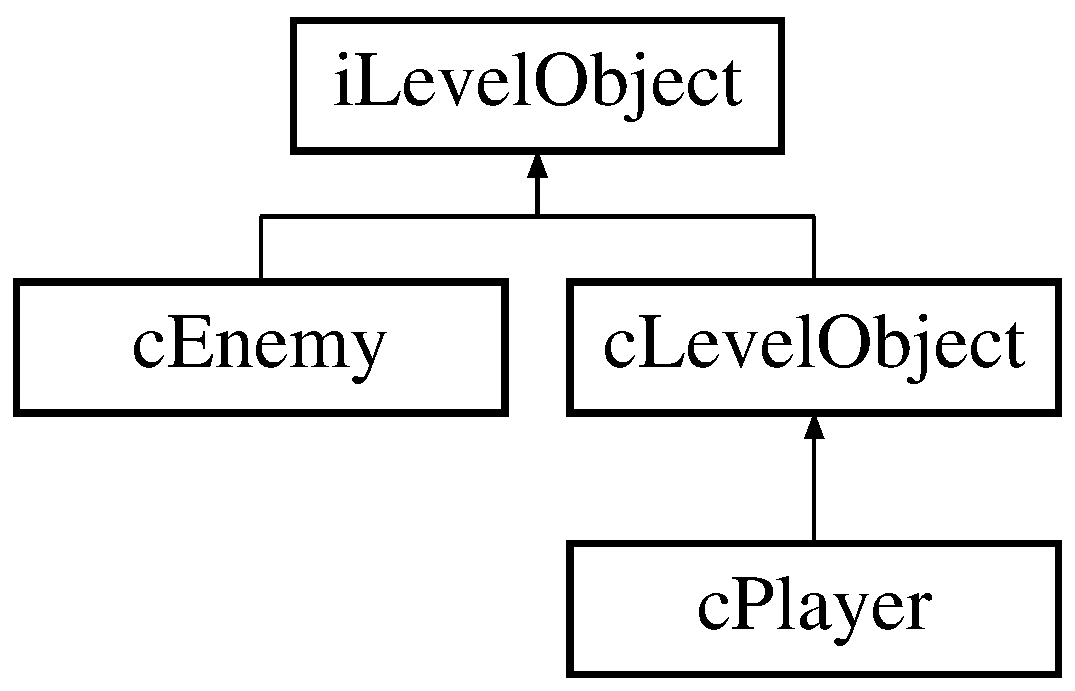
\includegraphics[height=3.000000cm]{classi_level_object}
\end{center}
\end{figure}
\subsection*{Public Member Functions}
\begin{DoxyCompactItemize}
\item 
\hypertarget{classi_level_object_a32b7a14285e0aa57eac94ab37bb0a7f1}{virtual void {\bfseries f\-Update} ()=0}\label{classi_level_object_a32b7a14285e0aa57eac94ab37bb0a7f1}

\end{DoxyCompactItemize}


The documentation for this class was generated from the following file\-:\begin{DoxyCompactItemize}
\item 
C\-:/\-Users/\-B\-W.\-K\-E\-E/\-Documents/\-Git\-Hub/\-Dungeon\-Brothers/ilevelobject.\-h\end{DoxyCompactItemize}

%--- End generated contents ---

% Index
\newpage
\phantomsection
\addcontentsline{toc}{part}{Index}
\printindex

\end{document}
